\documentclass{standalone}
\usepackage{tikz}
\usetikzlibrary{patterns, positioning}

\begin{document}
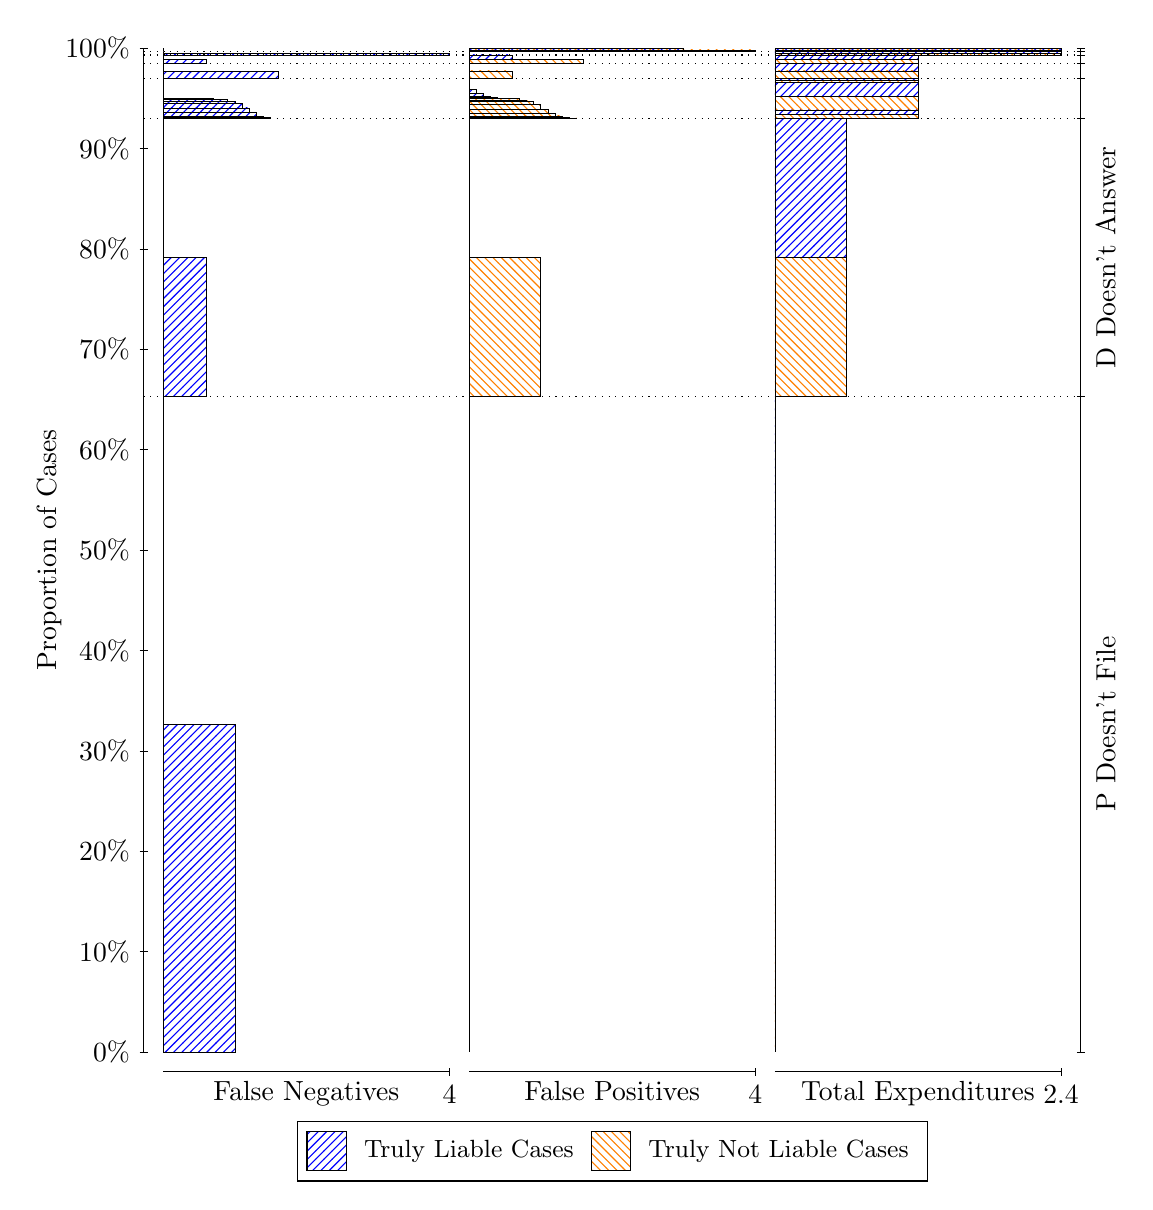
\begin{tikzpicture}
\draw[black, very thin] (1.5,1.75) -- (1.5,14.5);
\node[rotate=90, anchor=center] at (0.3, 8.125) {Proportion of Cases};
\draw[black, very thin] (1.45,1.75) -- (1.55,1.75);
\node[anchor=east] at (1.45, 1.75) {0\%};
\draw[black, very thin] (1.45,3.025) -- (1.55,3.025);
\node[anchor=east] at (1.45, 3.025) {10\%};
\draw[black, very thin] (1.45,4.3) -- (1.55,4.3);
\node[anchor=east] at (1.45, 4.3) {20\%};
\draw[black, very thin] (1.45,5.575) -- (1.55,5.575);
\node[anchor=east] at (1.45, 5.575) {30\%};
\draw[black, very thin] (1.45,6.85) -- (1.55,6.85);
\node[anchor=east] at (1.45, 6.85) {40\%};
\draw[black, very thin] (1.45,8.125) -- (1.55,8.125);
\node[anchor=east] at (1.45, 8.125) {50\%};
\draw[black, very thin] (1.45,9.4) -- (1.55,9.4);
\node[anchor=east] at (1.45, 9.4) {60\%};
\draw[black, very thin] (1.45,10.675) -- (1.55,10.675);
\node[anchor=east] at (1.45, 10.675) {70\%};
\draw[black, very thin] (1.45,11.95) -- (1.55,11.95);
\node[anchor=east] at (1.45, 11.95) {80\%};
\draw[black, very thin] (1.45,13.225) -- (1.55,13.225);
\node[anchor=east] at (1.45, 13.225) {90\%};
\draw[black, very thin] (1.45,14.5) -- (1.55,14.5);
\node[anchor=east] at (1.45, 14.5) {100\%};

\draw[black, very thin] (13.4,1.75) -- (13.4,14.5);
\draw[black, very thin] (13.35,1.75) -- (13.45,1.75);
\node[anchor=west] at (13.35, 1.75) {};
\draw[black, very thin] (13.35,10.078) -- (13.45,10.078);
\node[anchor=west] at (13.35, 10.078) {};
\draw[black, very thin] (13.35,13.605) -- (13.45,13.605);
\node[anchor=west] at (13.35, 13.605) {};
\draw[black, very thin] (13.35,14.111) -- (13.45,14.111);
\node[anchor=west] at (13.35, 14.111) {};
\draw[black, very thin] (13.35,14.306) -- (13.45,14.306);
\node[anchor=west] at (13.35, 14.306) {};
\draw[black, very thin] (13.35,14.412) -- (13.45,14.412);
\node[anchor=west] at (13.35, 14.412) {};
\draw[black, very thin] (13.35,14.456) -- (13.45,14.456);
\node[anchor=west] at (13.35, 14.456) {};
\draw[black, very thin] (13.35,14.5) -- (13.45,14.5);
\node[anchor=west] at (13.35, 14.5) {};

\draw[black, very thin, pattern color=blue, pattern=north east lines] (1.75,1.75) rectangle (2.6583,5.9142);
\draw[black, very thin, pattern color=orange, pattern=north west lines] (1.75,5.9142) rectangle (1.75,10.078);
\draw[black, very thin, pattern color=blue, pattern=north east lines] (1.75,10.078) rectangle (2.295,11.841);
\draw[black, very thin, pattern color=orange, pattern=north west lines] (1.75,11.841) rectangle (1.75,13.605);
\draw[black, very thin, pattern color=blue, pattern=north east lines] (1.75,13.605) rectangle (3.1125,13.622);
\draw[black, very thin, pattern color=blue, pattern=north east lines] (1.75,13.622) rectangle (3.0217,13.632);
\draw[black, very thin, pattern color=blue, pattern=north east lines] (1.75,13.632) rectangle (2.9308,13.679);
\draw[black, very thin, pattern color=blue, pattern=north east lines] (1.75,13.679) rectangle (2.84,13.74);
\draw[black, very thin, pattern color=blue, pattern=north east lines] (1.75,13.74) rectangle (2.7492,13.796);
\draw[black, very thin, pattern color=blue, pattern=north east lines] (1.75,13.796) rectangle (2.6583,13.826);
\draw[black, very thin, pattern color=blue, pattern=north east lines] (1.75,13.826) rectangle (2.5675,13.845);
\draw[black, very thin, pattern color=blue, pattern=north east lines] (1.75,13.845) rectangle (2.4767,13.852);
\draw[black, very thin, pattern color=blue, pattern=north east lines] (1.75,13.852) rectangle (2.3858,13.86);
\draw[black, very thin, pattern color=orange, pattern=north west lines] (1.75,13.86) rectangle (1.75,14.111);
\draw[black, very thin, pattern color=blue, pattern=north east lines] (1.75,14.111) rectangle (3.2033,14.207);
\draw[black, very thin, pattern color=orange, pattern=north west lines] (1.75,14.207) rectangle (1.75,14.306);
\draw[black, very thin, pattern color=blue, pattern=north east lines] (1.75,14.306) rectangle (2.295,14.359);
\draw[black, very thin, pattern color=orange, pattern=north west lines] (1.75,14.359) rectangle (1.75,14.412);
\draw[black, very thin, pattern color=blue, pattern=north east lines] (1.75,14.412) rectangle (5.3833,14.432);
\draw[black, very thin, pattern color=orange, pattern=north west lines] (1.75,14.432) rectangle (1.75,14.456);
\draw[black, very thin, pattern color=orange, pattern=north west lines] (1.75,14.456) rectangle (1.75,14.476);
\draw[black, very thin, pattern color=blue, pattern=north east lines] (1.75,14.476) rectangle (1.75,14.5);
\draw[black, very thin, pattern color=orange, pattern=north west lines] (5.6333,1.75) rectangle (5.6333,5.9142);
\draw[black, very thin, pattern color=blue, pattern=north east lines] (5.6333,5.9142) rectangle (5.6333,10.078);
\draw[black, very thin, pattern color=orange, pattern=north west lines] (5.6333,10.078) rectangle (6.5417,11.842);
\draw[black, very thin, pattern color=blue, pattern=north east lines] (5.6333,11.842) rectangle (5.6333,13.605);
\draw[black, very thin, pattern color=orange, pattern=north west lines] (5.6333,13.605) rectangle (6.9958,13.612);
\draw[black, very thin, pattern color=orange, pattern=north west lines] (5.6333,13.612) rectangle (6.905,13.62);
\draw[black, very thin, pattern color=orange, pattern=north west lines] (5.6333,13.62) rectangle (6.8142,13.638);
\draw[black, very thin, pattern color=orange, pattern=north west lines] (5.6333,13.638) rectangle (6.7233,13.668);
\draw[black, very thin, pattern color=orange, pattern=north west lines] (5.6333,13.668) rectangle (6.6325,13.723);
\draw[black, very thin, pattern color=orange, pattern=north west lines] (5.6333,13.723) rectangle (6.5417,13.782);
\draw[black, very thin, pattern color=orange, pattern=north west lines] (5.6333,13.782) rectangle (6.4508,13.828);
\draw[black, very thin, pattern color=orange, pattern=north west lines] (5.6333,13.828) rectangle (6.36,13.838);
\draw[black, very thin, pattern color=orange, pattern=north west lines] (5.6333,13.838) rectangle (6.2692,13.856);
\draw[black, very thin, pattern color=blue, pattern=north east lines] (5.6333,13.856) rectangle (6.0875,13.863);
\draw[black, very thin, pattern color=blue, pattern=north east lines] (5.6333,13.863) rectangle (5.9967,13.871);
\draw[black, very thin, pattern color=blue, pattern=north east lines] (5.6333,13.871) rectangle (5.9058,13.889);
\draw[black, very thin, pattern color=blue, pattern=north east lines] (5.6333,13.889) rectangle (5.815,13.92);
\draw[black, very thin, pattern color=blue, pattern=north east lines] (5.6333,13.92) rectangle (5.7242,13.976);
\draw[black, very thin, pattern color=blue, pattern=north east lines] (5.6333,13.976) rectangle (5.6333,14.111);
\draw[black, very thin, pattern color=orange, pattern=north west lines] (5.6333,14.111) rectangle (6.1783,14.21);
\draw[black, very thin, pattern color=blue, pattern=north east lines] (5.6333,14.21) rectangle (5.6333,14.306);
\draw[black, very thin, pattern color=orange, pattern=north west lines] (5.6333,14.306) rectangle (7.0867,14.358);
\draw[black, very thin, pattern color=blue, pattern=north east lines] (5.6333,14.358) rectangle (6.1783,14.412);
\draw[black, very thin, pattern color=orange, pattern=north west lines] (5.6333,14.412) rectangle (5.6333,14.436);
\draw[black, very thin, pattern color=blue, pattern=north east lines] (5.6333,14.436) rectangle (5.6333,14.456);
\draw[black, very thin, pattern color=orange, pattern=north west lines] (5.6333,14.456) rectangle (9.2667,14.476);
\draw[black, very thin, pattern color=blue, pattern=north east lines] (5.6333,14.476) rectangle (8.3583,14.5);
\draw[black, very thin, pattern color=orange, pattern=north west lines] (9.5167,1.75) rectangle (9.5167,5.9142);
\draw[black, very thin, pattern color=blue, pattern=north east lines] (9.5167,5.9142) rectangle (9.5167,10.078);
\draw[black, very thin, pattern color=orange, pattern=north west lines] (9.5167,10.078) rectangle (10.425,11.842);
\draw[black, very thin, pattern color=blue, pattern=north east lines] (9.5167,11.842) rectangle (10.425,13.605);
\draw[black, very thin, pattern color=orange, pattern=north west lines] (9.5167,13.605) rectangle (11.333,13.659);
\draw[black, very thin, pattern color=blue, pattern=north east lines] (9.5167,13.659) rectangle (11.333,13.715);
\draw[black, very thin, pattern color=orange, pattern=north west lines] (9.5167,13.715) rectangle (11.333,13.886);
\draw[black, very thin, pattern color=blue, pattern=north east lines] (9.5167,13.886) rectangle (11.333,14.059);
\draw[black, very thin, pattern color=orange, pattern=north west lines] (9.5167,14.059) rectangle (11.333,14.085);
\draw[black, very thin, pattern color=blue, pattern=north east lines] (9.5167,14.085) rectangle (11.333,14.111);
\draw[black, very thin, pattern color=orange, pattern=north west lines] (9.5167,14.111) rectangle (11.333,14.21);
\draw[black, very thin, pattern color=blue, pattern=north east lines] (9.5167,14.21) rectangle (11.333,14.306);
\draw[black, very thin, pattern color=orange, pattern=north west lines] (9.5167,14.306) rectangle (11.333,14.358);
\draw[black, very thin, pattern color=blue, pattern=north east lines] (9.5167,14.358) rectangle (11.333,14.412);
\draw[black, very thin, pattern color=orange, pattern=north west lines] (9.5167,14.412) rectangle (13.15,14.436);
\draw[black, very thin, pattern color=blue, pattern=north east lines] (9.5167,14.436) rectangle (13.15,14.456);
\draw[black, very thin, pattern color=orange, pattern=north west lines] (9.5167,14.456) rectangle (13.15,14.476);
\draw[black, very thin, pattern color=blue, pattern=north east lines] (9.5167,14.476) rectangle (13.15,14.5);
\draw[black, dotted] (1.5,10.078) -- (13.4,10.078);
\draw[black, dotted] (1.5,13.605) -- (13.4,13.605);
\draw[black, dotted] (1.5,14.111) -- (13.4,14.111);
\draw[black, dotted] (1.5,14.306) -- (13.4,14.306);
\draw[black, dotted] (1.5,14.412) -- (13.4,14.412);
\draw[black, dotted] (1.5,14.456) -- (13.4,14.456);
\draw[black, very thin] (1.75,1.5) -- (5.3833,1.5);
\node[anchor=north] at (3.5667, 1.5) {False Negatives};
\draw[black, very thin] (5.3833,1.45) -- (5.3833,1.55);
\node[anchor=north] at (5.3833, 1.45) {4};

\draw[black, very thin] (5.6333,1.5) -- (9.2667,1.5);
\node[anchor=north] at (7.45, 1.5) {False Positives};
\draw[black, very thin] (9.2667,1.45) -- (9.2667,1.55);
\node[anchor=north] at (9.2667, 1.45) {4};

\draw[black, very thin] (9.5167,1.5) -- (13.15,1.5);
\node[anchor=north] at (11.333, 1.5) {Total Expenditures};
\draw[black, very thin] (13.15,1.45) -- (13.15,1.55);
\node[anchor=north] at (13.15, 1.45) {2.4};

\node[black, centered, rotate=90] at (13.72, 5.9142) {P Doesn't File};
\node[black, centered, rotate=90] at (13.72, 11.842) {D Doesn't Answer};






\draw (7.449999999999999,1.5) node[draw=none] (baseCoordinate) {};
\begin{scope}[align=center]
        \matrix[scale=0.5, draw=black, below=0.5cm of baseCoordinate, nodes={draw}, column sep=0.1cm]{
            \node[rectangle, draw, minimum width=0.5cm, minimum height=0.5cm, pattern=north east lines, pattern color=blue] {}; &
            \node[draw=none, font=\small] (B) {Truly Liable Cases}; &
            \node[rectangle, draw, minimum width=0.5cm, minimum height=0.5cm, pattern=north west lines, pattern color=orange] {}; &
            \node[draw=none, font=\small] (B) {Truly Not Liable Cases}; \\
            };
\end{scope}

\end{tikzpicture}
\end{document}